\documentclass[10pt,a4paper,leqno]{article}
\usepackage[utf8]{inputenc}
\usepackage{amsmath}
\usepackage{amsfonts}
\usepackage{amssymb}

\usepackage{multirow}
\usepackage[table,xcdraw]{xcolor}

\addtolength{\oddsidemargin}{-.5in}
\addtolength{\evensidemargin}{-.5in}
\addtolength{\textwidth}{1in}

\addtolength{\topmargin}{-.5in}
\addtolength{\textheight}{1in}

\usepackage{setspace}
\usepackage{graphicx}

\newcommand{\dcell}{D_{\text{cell}}}
\newcommand{\urow}{U_{\text{row}}}

\newcommand{\ucol}{U_{\text{column}}}
\newcommand{\ublock}{U_{\text{block}}}

\newcommand{\ucell}{U_{\text{cell}}}
\newcommand{\drow}{D_{\text{row}}}

\newcommand{\dcol}{D_{\text{column}}}
\newcommand{\dblock}{D_{\text{block}}}

\newcommand{\lp}{\left(}
\newcommand{\rp}{\right)}

\begin{document}

\title{SAT Solving Sudokus with Encoded Redundancies and Human Strategies \\
Knowledge Presentation - Project 1}
\author{Pasquale Muscettola, Mathijs Mul}
\maketitle

\section*{Hypothesis}

%The Sudoku game is defined by a set of rules that can be considered as constraints on the admissible set of number assignments in the grid. These constraints depend on the distribution of the set of available numbers over the spatial units that are identified. Traditionally, $n^2$ rows, columns and blocks are distinguished, each of  which contain a total of $n^2$ cells, where $n =3$ is most conventional. In this paper, we will focus on this standard Sudoku format, whose solution requires the numbers 1 to 9 to be placed once and only once in each row, column and block. 

Logically, the constraints governing the Sudoku game can be considered as a set of axioms, which allow for the inference from an initial assignment of given numbers to a completely filled out grid through a number of intermediate reasoning steps. Each configuration of numbers that follows from the given assignment in accordance with the rules of the game can thus be seen as a 'theorem' of the particular Sudoku. Continuing this logic is eventually supposed to culminate in a correct solution to the puzzle. Taking this logical approach on the traditional $n = 3$ Sudoku format, we will investigate different possible encodings of the game constraints in Propositional Logic. After identifying the minimal set of constraints that are necessary and sufficient in characterising the game, we will identify several extensions and variations. Using a SAT solver we will then study how the different and extended encodings influence the computational effort that is needed to solve puzzles that have been indicated to be of the same (human) difficulty rate on an online database. 

Thus, what we will do is look at alternative Sudoku encodings that are logically implied by the minimal set of constraints, and that could thus be considered redundant from a purely syntactic point of view. In particular, we wish to look at techniques that human solvers use to address Sudoku puzzles, formalize such strategies and add them to the encoding to study how this influences the required computational effort. Logically, such strategies could also be considered superfluous, as they follow from the general axioms and thus provide no new information. An interest in the difference between the computational and the logical impact of adding such redundancies is the main motivation for this research. 

We hypothesize that \textbf{adding redundant clauses to the encoding of the Sudoku game, in the form of trivial logical extensions and human strategies, will decrease the computational effort needed by a SAT engine to find a solution}. Even though such propositions are implied by the minimal set of constraints characterising the game, so that they are logically redundant, we expect that including them in the propositional representation of the game will lead to computational speed-up. Our main reason for believing this is that adding constraints decreases the search space for a SAT solver, and should thus speed up the computation. 

\section*{Experimental setup}

%describe it, motivate/justify it, discuss possible weaknesses or problems, how do you compensate for those. What dataset did you use, which metrics did you use, which variables did you vary, etc. 
 
In order to test our hypothesis we used a large database of Sudokus from the website www.thonky.com, which are rated according to their difficulty as perceived by human solvers. We used the SAT solver zChaff to solve the puzzles, which comprises a deterministic algorithm that has achieved very well in SAT competitions and that provides clear statistical information with its output. 

The notion of computational effort at stake in this project is identified as the number of decisions that have to be made by zChaff in order to complete a Sudoku puzzle. This is our metric of computational `hardness'. We chose not to base our conclusions on runtime, mainly because solving a Sudoku can be done very quickly by zChaff, so that the required time is in a range that is too sensitive to irrelevant background processes in the computer to be an accurate indication of underlying computational effort. However, as we considered a large collection of puzzles, we still looked at relative differences in runtime between different cases. 

Before running any tests, we had to determine the different kinds of encodings of Sudoku puzzles that we wished to consider. In this, we decided to focus on three cases: one where we only work with the minimal set of constraints that are necessary and sufficient for characterising the game, a second one that uses a trivial extension of this minimal encoding, and a third one that incorporates the propositionalization of a human solving strategy. 

First, the minimal propositional encoding of the Sudoku puzzle must be determined. This only requires the basic constraints, which on their own are enough to define the game, namely:

\begin{itemize}

\item $\dcell$: \textbf{Definedness of cells}: all cells in the grid should contain at least one value from the set $\{i | 1 \leq i \leq n^2\}$.

\item $\urow$: \textbf{Uniqueness in rows}: in each row, all values from the set $\{i | 1 \leq i \leq n^2\}$ should feature at most once. 

\item $\ucol$: \textbf{Uniqueness in columns}: idem for columns. 

\item $\ublock$: \textbf{Uniqueness in blocks}: idem for blocks.

\item $N_{\text{assigned}}$ : \textbf{Assigned numbers}: the numbers given in the Sudoku grid cannot be changed. 

\end{itemize}

In order to give an adequate representation in propositional logic, we define $(n^2)^3$ variables of the form $(r,c,v)$, where $r$ denotes row number, $c$ denotes column number and $v$ denotes number value of the cell whose location in the grid is specified by $r$ and $c$. With these variables we can formulate the following propositional encoding of the above-mentioned constraints:  

\begin{itemize}

\item $\dcell$: 
$\bigwedge_{r=1}^{n^2} \bigwedge_{c=1}^{n^2} \bigvee_{v=1}^{n^2} (r,c,v)$

\item $\urow$:
$\bigwedge_{r=1}^{n^2} \bigwedge_{v=1}^{n^2}\bigwedge_{c_i=n}^{n^2 - 1} \bigwedge_{c_j=c_i+1}^{n^2} \neg(r,c_i,v) \lor \neg(r,c_j,v)$


\item $\ucol$: 
$\bigwedge_{c=1}^{n^2} \bigwedge_{v=1}^{n^2}\bigwedge_{r_i=n}^{n^2-1} \bigwedge_{r_j=r_i+1}^{n^2} \neg(r_i,c,v) \lor \neg(r_j,c,v)$


\item $\ublock$:  
$\bigwedge_{r_{\text{block}} = 1}^{n} \bigwedge_{c_{\text{block}} = 1}^{n}\bigwedge_{v=1}^{n^2} \bigwedge_{r = 1}^{n^2} \bigwedge_{c = r + 1}^{n^2} \neg(r_{\text{block}} n + r \mod n,c_{\text{block}} n + r \mod n,v) \lor \neg(r_{\text{block}} n + c \mod n,c_{\text{block}} n + c \mod n,v)$

\item $N_{\text{assigned}}$ : 
$\bigwedge_{\text{Assigned}} (r,c,v)$ for Assigned = $\{ (r,c,v) | (r,c,v) $ is given$\}$.


\end{itemize}

We let $E_{\text{minimal}} = \{\dcell,\urow,\ucol,\ublock, N_{\text{assigned}}\}$ denote the minimal encoding. From this minimal set of constraints, we can derive some other constraints, which will be added as redundancies. The most elementary redundancies to consider are the following: 


\begin{itemize}

\item $\ucell$: \textbf{Uniqueness of cells}: all cells in the grid should contain at most one value from the set $\{i | 1 \leq i \leq n^2\}$.

\item $\drow$: \textbf{Definedness in rows}: in each row, all values from the set $\{i | 1 \leq i \leq n^2\}$ should feature at least once. 

\item $\dcol$: \textbf{Definedness in columns}: idem for columns. 

\item $\dblock$: \textbf{Definedness in blocks}: idem for blocks. 

\end{itemize}

Propositional encoding is as follows: 

\begin{itemize}

\item $\ucell$: 
$\bigwedge_{r=1}^{n^2} \bigwedge_{c=1}^{n^2}\bigwedge_{v_i=n}^{n^2 - 1} \bigwedge_{v_j=v_i+1}^{n^2} \neg(r,c,v_i) \lor \neg(r,c,v_j)$


\item $\drow$:
$\bigwedge_{r=1}^{n^2} \bigwedge_{v=1}^{n^2} \bigvee_{c=1}^{n^2} (r,c,v)$

\item $\dcol$: 
$\bigwedge_{c=1}^{n^2} \bigwedge_{v=1}^{n^2} \bigvee_{r=1}^{n^2} (r,c,v)$

\item $\dblock$:  
$\bigwedge_{r_{\text{block}} = 1}^{n} \bigwedge_{c_{\text{block}} = 1}^{n}\bigwedge_{v=1}^{n^2} \bigvee_{r = 1}^{n} \bigvee_{c = 1}^{n} (r_{\text{block}} n + r ,c_{\text{block}} n +c,v) $

\end{itemize}

We let $E_{\text{extended}} = E_{\text{minimal}} \cup \{\ucell,\drow,\dcol,\dblock\}$ denote the extended encoding comprising the minimal constraints in addition to the redundancies listed above. 

In addition to the extension thus defined, we are interested in human Sudoku solving techniques, i.e. so-called `pencil and paper' algorithms that are usually applied intuitively and informally. Such strategies could also be seen as logical consequences of $E_{\text{minimal}}$. Strictly speaking, they add no new information, but by efficient filtering of the infinitely many implications of the basic Sudoku axioms, they do make solving the puzzles easier. We want to encode such a strategy, add it to the propositional Sudoku representation and study how this impacts the computational effort needed by zChaff to find solutions. According to our hypothesis, extending the encoding with such information should make computation easier, not only for a human solver, but also for a SAT solver.

In particular, we decided to look at the so-called `Naked Twins' strategy, as it is a basic and well-known human Sudoku solving method. The strategy makes use of an exclusion rule that can be described and formalised as follows:

\begin{itemize}

\item $ R_{\text{NT}}$: \textbf{Naked Twins}: if two cells in a unit are such that together they must contain two specific numbers, but the order is unknown, then no other cells in this unit should contain either of of these numbers. If we consider the row units, then the propositional formalisation is as follows: 
 
$\bigwedge_{r=1}^{n^2} \bigwedge_{c_1=1}^{n^2-1}\bigwedge_{c_2=c_1 + 1}^{n^2} \bigwedge_{v_1=1}^{n^2 - 1} \bigwedge_{v_2=v_1 + 1}^{n^2} \bigwedge_{c_3 \neq c_1,c_2} $

$\;\;\;\;\;\;\;\;\;\;\;\; \lp \bigvee_{v_3 \neq v_1,v_2} \lp (r,c_1,v_3) \lor (r,c_2,v_3)\rp \lor \neg (r,c_3,v_1) \rp 
\wedge
\lp \bigvee_{v_3 \neq v_1,v_2} \lp (r,c_1,v_3) \lor (r,c_2,v_3)\rp \lor \neg (r,c_3,v_2) \rp 
$

The Naked Twins strategy can be applied to columns as well, the propositional formalisation of which is completely analogous to the one for row, so we omit it here.

\end{itemize}

We let $R_{\text{NT-row}}$, $R_{\text{NT-column}}$ denote Naked Twins rule for rows and columns respectively, and let $E_{\text{strategy}} = E_{\text{extended}} \cup \{R_{\text{NT-row}}, R_{\text{NT-column}}\}$ be the extended encoding that also includes a representation of this strategy. 
\footnote{
An alternative human strategy that we encoded involved iterating over all possible permutations of $n^2 - 1$ numbers in each unit, and resulted in a CNF file that was more than 1 GB in size. This proved impossible to work with, and only gave segmentation faults when passed to the SAT solver, so we had to exclude it from the experiment.}

With all definitions set up, the actual experiment was as follows: for each of three classes of human-rated difficulty degrees (easy, medium, hard), we extracted 100 Sudokus from our database, and let zChaff solve them for all three encodings $E_{\text{minimal}}, E_{\text{extended}} $ and $E_{\text{strategy}} $. We collected the data and studied the differences between the number of decisions required to solve the puzzle, the results of which are demonstrated in the next section. 

The Sudokus in our dataset have a human difficulty rating, which we realized may be subject to debate and different experiences. To compensate for this, we used 100 Sudokus of every difficulty class, a number that we believed should be high enough to stabilize this factor. 

Moreover, we only considered proper Sudokus, because improper ones require the solver to make a non-deterministic decision at some point, which is an action that cannot be accounted for on the basis of the minimal set of rules captured by $E_{\text{minimal}}$ that we considered as a definition of the game. This set is also most common for human pencil and paper puzzles, and as we are mainly interested in drawing the comparison between human and computational effort, we decided not to deviate from it. 


\section*{Experimental results}

%describe your experimental findings, discuss if they are reliable etc.
 
Running the experiment as described in the above yielde the following results, where all values are averaged over the 100 test Sudokus for each difficulty category:


\begin{table}[]
\centering
\caption{Results}
\label{my-label}
\begin{tabular}{|
>{\columncolor[HTML]{FFFFFF}}c |
>{\columncolor[HTML]{FFFFFF}}c |
>{\columncolor[HTML]{FFFFFF}}c |
>{\columncolor[HTML]{FFFFFF}}c |
>{\columncolor[HTML]{FFFFFF}}c |
>{\columncolor[HTML]{FFFFFF}}c |}
\hline
human difficulty & encoding              & decision level & number of decisions & runtime     & number of implications \\ \hline
                 & $E_{\text{minimal}}$  & 10.8438        & 42.0859             & 0.000737133 & 1959.81                \\ \cline{2-6} 
easy             & $E_{\text{extended}}$ & 0.625          & 1.82812             & 0.000481484 & 743.125                \\ \cline{2-6} 
                 & $E_{\text{strategy}}$ & 0.716535       & 2.02362             & 0.0543418   & 758.858                \\ \hline
                 & $E_{\text{minimal}}$  & 12.0515        & 53.8515             & 0.000940952 & 2349.26                \\ \cline{2-6} 
medium           & $E_{\text{extended}}$ & 1.61515        & 3.28182             & 0.000484706 & 758.967                \\ \cline{2-6} 
                 & $E_{\text{strategy}}$ & 1.13982        & 2.79635             & 0.0554446   & 766.167                \\ \hline
                 & $E_{\text{minimal}}$  & 12.883         & 57.1585             & 0.00098467  & 2497.61                \\ \cline{2-6} 
hard             & $E_{\text{extended}}$ & 2.04528        & 3.84717             & 0.000502104 & 785.432                \\ \cline{2-6} 
                 & $E_{\text{strategy}}$ & 1.30624        & 3.23819             & 0.0592149   & 810.684                \\ \hline
\end{tabular}
\end{table}



We provide the following visualizations:


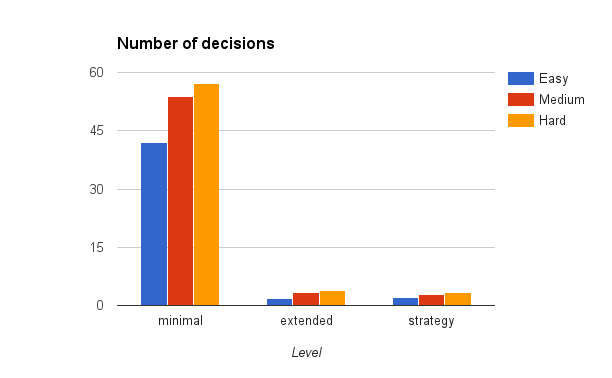
\includegraphics[scale=0.5]{chart_decisions.png}


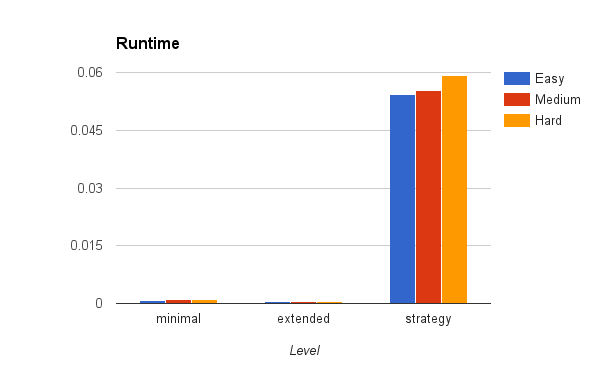
\includegraphics[scale=0.5]{chart_runtime.png}

 

\section*{Interpretation}

%what do your experimental results say about your hypothesis, do they confirm or falsify your hypothesis, do they show any further interesting lessons

Our results, and especially the visualized number of decisions, show clearly that the minimal encoding requires the SAT solver to make a significantly higher number of decisions than the extended and strategy encodings. This holds for all human difficulty degrees that we considered. Indeed, after extending $E_{\text{minimal}}$ to $E_{\text{extended}}$ the number of necessary decisions is already drastically reduced, and the extra encoding of the Naked Twins strategy does not lead to a significant improvement on top of this. In general, we can say that the results show that adding logically redundant constraints to the Sudoku encoding significantly reduces the computational effort required by zChaff to find a solution, irrespective of the human difficulty rating. This is in accordance with our hypothesis. 

Some other interesting finding, that we did not decide to focus on in the research but that emerged from the statistical results, is that the runtime develops in the opposite direction: for $E_{\text{minimal}}$ to $E_{\text{extended}}$ it is of comparable order of magnitude, whereas for $E_{\text{strategy}}$ it increases dramatically. Thus, although encoding the Naked Twins strategy reduces the required number of decisions, and thus decreases computational effort as we decided to regard it, it does not decrease the needed runtime. In fact, the runtime becomes much higher. This can be explained by the great increase of the number of clauses in the encoding  $E_{\text{strategy}}$: the high number of constraints necessitates very few decisions, but because the CNF becomes so large, the runtime grows. 


\section*{Conclusion} 

%summary, future work: summarise your work and conclusions, and suggest new tasks or questions that follow from your work. 

In summary, we can conclude that our experiment has confirmed our hypothesis: adding redundant clauses to the minimal Sudoku encoding in propositional logic reduces the computational effort required by the SAT solver zChaff to find a solution, as measured in terms of the number of decisions. Moreover, this finding is robust for different human difficulty ratings: we see the same relationship for puzzles that were evaluated as easy, medium and hard. 

However, encoding the human pencil and paper strategy of Naked Twins does not give significant computational benefits on top of the more or less trivial extension $E_{\text{extended}}$. So apparently this human strategy is of less computational interest for zChaff than the basic extension. This also shows that means of reducing the required human effort to solve a Sudoku puzzle, such as this strategy, do not necessarily entail great computational benefits for SAT solvers. 

Our research has triggered many other questions. Obviously, it would be very relevant to consider the encodings of different human solving strategies, and compare the effects of different methods on the achievements of a SAT solver. Also, it would be worthwhile to investigate whether our results are robust across SAT solvers. zChaff is deterministic, but comparison with non-deterministic algorithms would be interesting. We could also consider variations with respect to the Sudokus in our data set. For example, it is possible to look at improper Sudokus and see what this would imply for different encodings. Also, we could upscale the Sudokus on which we tested, and study larger ones with $n=4$ or more. 



\end{document}